%%%%%%%%%%%%%%%%%%%%%%%% INICIO QUADRO 01 %%%%%%%%%%%%%%%%%%%%%%%%%%%%%%%
\begin{table}[ht]
  \centering
  \caption{Quadro 01}
  \label{Quadro_01}
  \begin{tabular}[t]{|p{2.6cm}|l|l|l|}
    \hline

    %%% PRÓXIMA LINHA
    \letraquadrada{A}   &   \letraquadrada{A1}    &    \letraquadrada{B}    &    \letraquadrada{C}


    %%% PRÓXIMA LINHA
    \\
    \quadtitulo{Clave de Percussão}
    &
    \quadtitulo{Semínimas}
    &
    \quadtitulo{Compasso}
    &
    \quadtitulo{Fórmula de compasso}


    %%% PRÓXIMA LINHA
    \\
    \includegraphics[scale=1]{clave-percussao}
    &
    \includegraphics[scale=1]{per-seminimas}
    &
    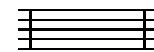
\includegraphics[scale=1]{compasso-vazio}
    &
    \includegraphics[scale=1]{4tempos-por-compasso}


    %%% PRÓXIMA LINHA
    \\
    \hline
    \multicolumn{2}{|l|}{\letraquadrada{D}}
    &
    \letraquadrada{E}
    &
    \letraquadrada{F}


    %%% PRÓXIMA LINHA
    \\
    \multicolumn{2}{|l|}{\quadtitulo{Semibreve}}
    &
    \quadtitulo{Mínima}
    &
    \quadtitulo{Pausa de semibreve}


    %%% PRÓXIMA LINHA
    \\
    \multicolumn{2}{|l|}{\includegraphics[scale=1]{semibreve}}
    &
    \includegraphics[scale=1]{minima}
    &
    \includegraphics[scale=1]{semibreve-pausa}



    %%% FINAL DAS LINHAS
  \\
  \hline
  \end{tabular}
\end{table}    


%%%%%%%%%%%%%%%%%%%%%%%% FINAL QUADRO %%%%%%%%%%%%%%%%%%%%%%%%%%%%%%%%%%%


%%%%%%%%%%%%%%%%%%%%%%%% INICIO QUADRO 02 %%%%%%%%%%%%%%%%%%%%%%%%%%%%%%%

\begin{table}[ht]
  \centering
  \caption{Quadro 02}
  \label{Quadro_02}
  \begin{tabular}[t]{|l|l|l|}
    \hline

    %%% PRÓXIMA LINHA
    \letraquadrada{A}    &    \letraquadrada{B}    &    \letraquadrada{C}


    %%% PRÓXIMA LINHA
    \\
    \quadtitulo{Pausa de mínima}
    &
    \quadtitulo{Barra final}
    &
    \quadtitulo{Barra de compasso}


    %%% PRÓXIMA LINHA
    \\
    \includegraphics[scale=1]{minima-pausa}
    &
    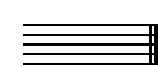
\includegraphics[scale=1]{barra-final}
    &
    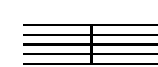
\includegraphics[scale=1]{barra-compasso}


    %%% PRÓXIMA LINHA
    \\
    \hline
    \letraquadrada{D}
    &
    \letraquadrada{E}
    &
    \letraquadrada{F}


    %%% PRÓXIMA LINHA
    \\
    \quadtitulo{Semínima}
    &
    \quadtitulo{Fórmula de compasso}
    &
    \quadtitulo{Batidas Alternadas}


    %%% PRÓXIMA LINHA
    \\
    \includegraphics[scale=1]{seminima}
    &
    \includegraphics[scale=1]{formula-4tempos-por-compasso}
    &
    \includegraphics[scale=1]{per-batidas-alternadas}


    %%% FINAL DAS LINHAS
  \\
  \hline
  \end{tabular}
\end{table}    



%%%%%%%%%%%%%%%%%%%%%%%% FINAL QUADRO %%%%%%%%%%%%%%%%%%%%%%%%%%%%%%%%%%%


%%%%%%%%%%%%%%%%%%%%%%%% INICIO QUADRO 03 %%%%%%%%%%%%%%%%%%%%%%%%%%%%%%%

\begin{table}[ht]
  \centering
  \caption{Quadro 03}
  \label{Quadro_03}
  \begin{tabular}[t]{|l|l|l|}
    \hline

    %%% PRÓXIMA LINHA
    \letraquadrada{A}    &    \letraquadrada{B}    &    \letraquadrada{C}


    %%% PRÓXIMA LINHA
    \\
    \quadtitulo{Batidas Duplas}
    &
    \quadtitulo{Sinal de respiração}
    &
    \quadtitulo{Pauta ou pentagrama}


    %%% PRÓXIMA LINHA
    \\
    \includegraphics[scale=1]{per-batidas-duplas}
    &
    \includegraphics[scale=1]{respiracao}
    &
    \includegraphics[scale=1]{pauta}



    %%% FINAL DAS LINHAS
  \\
  \hline
  \end{tabular}
\end{table}    


%%%%%%%%%%%%%%%%%%%%%%%% FINAL QUADRO %%%%%%%%%%%%%%%%%%%%%%%%%%%%%%%%%%%


%%%%%%%%%%%%%%%%%%%%%%%% INICIO QUADRO 04 %%%%%%%%%%%%%%%%%%%%%%%%%%%%%%%

\begin{table}[ht]
  \centering
  \caption{Quadro 04}
  \label{Quadro_04}
  \begin{tabular}[t]{|l|l|l|}
    \hline

    %%% PRÓXIMA LINHA
    \letraquadrada{A}    &    \letraquadrada{B}    &    \letraquadrada{C}


    %%% PRÓXIMA LINHA
    \\
    \quadtitulo{Paradidle simples}
    &
    \quadtitulo{Pausa de semínima}
    &
    \quadtitulo{Fórmula de compasso}


    %%% PRÓXIMA LINHA
    \\
    \includegraphics[scale=1]{per-paradidle-simples}
    &
    \includegraphics[scale=1]{seminima-pausa}
    &
    \includegraphics[scale=1]{formula-3tempos-por-compasso}


    %%% FINAL DAS LINHAS
    \\
    \hline
  \end{tabular}

  \begin{tabular}[t]{|l|l|}
    %%% PRÓXIMA LINHA

    \letraquadrada{D}
    &
    \letraquadrada{E}
   

    %%% PRÓXIMA LINHA
    \\
    \quadtitulo{Clave de sol}
    &
    \quadtitulo{Clave de fá}


    %%% PRÓXIMA LINHA
    \\
    \includegraphics[scale=1]{clave-sol}
    &
    \includegraphics[scale=1]{clave-fa}

    %%% FINAL DAS LINHAS
  \\
  \hline
  \end{tabular}
\end{table}    

%%%%%%%%%%%%%%%%%%%%%%%% FINAL QUADRO %%%%%%%%%%%%%%%%%%%%%%%%%%%%%%%%%%%

%%%%%%%%%%%%%%%%%%%%%%%% INICIO QUADRO 05 %%%%%%%%%%%%%%%%%%%%%%%%%%%%%%%

\begin{table}[ht]
  \centering
  \caption{Quadro 05}
  \label{Quadro_05}
  \begin{tabular}[t]{|p{4.5cm}|l|l|}
    \hline

    %%% PRÓXIMA LINHA
    \letraquadrada{A}    &    \letraquadrada{B}    &    \letraquadrada{C}


    %%% PRÓXIMA LINHA
    \\
    \quadtitulo{Triângulo}
    &
    \quadtitulo{Ligadura}
    &
    \quadtitulo{Fórmula de compasso}


    %%% PRÓXIMA LINHA
    \\
    \quadtexto{Tocar suspendendo-o em um pedaço de linha ou couro,
      usando a sua baqueta específica e batendo no ângulo oposto ao
      ângulo aberto}
    &
    \includegraphics[scale=1]{ligadura-minima}
    &
    \includegraphics[scale=1]{formula-2tempos-por-compasso}


    %%% FINAL DAS LINHAS
    \\
    \hline
  \end{tabular}

  \begin{tabular}[t]{|l|l|}
    %%% PRÓXIMA LINHA

    \letraquadrada{D}
    &
    \letraquadrada{E}
   

    %%% PRÓXIMA LINHA
    \\
    \quadtitulo{Andamento}
    &
    \quadtitulo{Anacruse}


    %%% PRÓXIMA LINHA
    \\
    \includegraphics[scale=1]{andamento}
    &
    \includegraphics[scale=1]{anacruse5}

    %%% FINAL DAS LINHAS
  \\
  \hline
  \end{tabular}
\end{table}    

%%%%%%%%%%%%%%%%%%%%%%%% FINAL QUADRO %%%%%%%%%%%%%%%%%%%%%%%%%%%%%%%%%%%

%%%%%%%%%%%%%%%%%%%%%%%% INICIO QUADRO 06 %%%%%%%%%%%%%%%%%%%%%%%%%%%%%%%

\begin{table}[ht]
  \centering
  \caption{Quadro 06}
  \label{Quadro_06}
  \begin{tabular}[t]{|l|l|}
    \hline

    %%% PRÓXIMA LINHA
    \letraquadrada{A}    &    \letraquadrada{B}


    %%% PRÓXIMA LINHA
    \\
    \em
    &
    \quadtitulo{Sinal de repetição}


    %%% PRÓXIMA LINHA
    \\
    \begin[fragment]{lilypond}
      \transpose c c {
        \keepWithTag #'cl
        \include "descanso.ly"
      }
    \end{lilypond}
    &
    \includegraphics[scale=1]{sinal-repeticao}


    %%% PRÓXIMA LINHA
    \\
    \hline
    \multicolumn{2}{|l|}{\letraquadrada{C}}

    %%% PRÓXIMA LINHA
    \\
    \multicolumn{2}{|l|}{\quadtitulo{Anacruse}}


    %%% PRÓXIMA LINHA
    \\
    \multicolumn{2}{|c|}{\includegraphics[scale=1]{anacruse6}}


    %%% FINAL DAS LINHAS
    \\
    \hline
  \end{tabular}
\end{table}    


%%%%%%%%%%%%%%%%%%%%%%%% FINAL QUADRO %%%%%%%%%%%%%%%%%%%%%%%%%%%%%%%%%%%

%%%%%%%%%%%%%%%%%%%%%%%% INICIO QUADRO 07 %%%%%%%%%%%%%%%%%%%%%%%%%%%%%%%

\begin{table}[ht]
  \centering
  \caption{Quadro 07}
  \label{Quadro_07}
  \begin{tabular}[t]{|l|l|l|}
    \hline

    %%% PRÓXIMA LINHA
    \letraquadrada{A}    &    \letraquadrada{B}    &    \letraquadrada{C}


    %%% PRÓXIMA LINHA
    \\
    \em
    &
    \quadtitulo{Sinal de repetição}
    &
    \quadtitulo{Moderato}


    %%% PRÓXIMA LINHA
    \\
    \begin[fragment]{lilypond}
      \transpose c c {
        \keepWithTag #'cl
        \include "descanso.ly"
      }
    \end{lilypond}
    &
    \includegraphics[scale=1]{sinal-repeticao7-1}
    &
    \includegraphics[scale=1]{moderato}


    %%% PRÓXIMA LINHA
    \\
    \em
    &
    \includegraphics[scale=1]{sinal-repeticao7-2}
    &
    \em

    %%% FINAL DAS LINHAS
    \\
    \hline
  \end{tabular}
\end{table}    

%%%%%%%%%%%%%%%%%%%%%%%% FINAL QUADRO %%%%%%%%%%%%%%%%%%%%%%%%%%%%%%%%%%%

%%%%%%%%%%%%%%%%%%%%%%%% INICIO QUADRO 08 %%%%%%%%%%%%%%%%%%%%%%%%%%%%%%%

\begin{table}[ht]
  \centering
  \caption{Quadro 08}
  \label{Quadro_08}
  \begin{tabular}[t]{|l|l|l|}
    \hline

    %%% PRÓXIMA LINHA
    \letraquadrada{A}    &    \letraquadrada{B}    &    \letraquadrada{C}


    %%% PRÓXIMA LINHA
    \\
    \em
    &
    \quadtitulo{Ponto de aumento}
    &
    \quadtitulo{Ligadura de prolongação}


    %%% PRÓXIMA LINHA
    \\
    \begin[fragment]{lilypond}
      \transpose c c {
        \keepWithTag #'cl
        \include "descanso.ly"
      }
    \end{lilypond}
    &
    \includegraphics[scale=1]{minima-pontuada}
    &
    \includegraphics[scale=1]{minima-ligada-seminima}



    %%% FINAL DAS LINHAS
    \\
    \hline
  \end{tabular}

  \begin{tabular}[t]{|l|p{7cm}|}
    %%% PRÓXIMA LINHA

    \letraquadrada{D}
    &
    \letraquadrada{E}
   

    %%% PRÓXIMA LINHA
    \\
    \quadtitulo{Ambos os sis são bemóis}
    &
    \quadtitulo{Armadura de clave de mi bemol maior}


    %%% PRÓXIMA LINHA
    \\
    \includegraphics[scale=1]{clave-sol-sis-bemois}
    &
    \begin[fragment]{lilypond}
      \override Staff.TimeSignature #'transparent = ##t
      \key ees \major
      s
    \end{lilypond}
    \quadtexto{Indica que as notas si, mi e lá são bemóis.}


    %%% FINAL DAS LINHAS
  \\
  \hline
  \end{tabular}
\end{table}    

%%%%%%%%%%%%%%%%%%%%%%%% FINAL QUADRO %%%%%%%%%%%%%%%%%%%%%%%%%%%%%%%%%%%


%%%%%%%%%%%%%%%%%%%%%%%% INICIO QUADRO 09 %%%%%%%%%%%%%%%%%%%%%%%%%%%%%%%

\begin{table}[ht]
  \centering
  \caption{Quadro 09}
  \label{Quadro_09}
  \begin{tabular}[t]{|c|}
    \hline

    %%% PRÓXIMA LINHA
    \quadtitulo{Compassos de espera}


    %%% PRÓXIMA LINHA
    \\
    \includegraphics[scale=1]{8compassos-pausa}

    %%% PRÓXIMA LINHA
    \\
    \quadtexto{8 compassos de pausa}

  \\
  \hline
  \end{tabular}
\end{table}    

%%%%%%%%%%%%%%%%%%%%%%%% FINAL QUADRO %%%%%%%%%%%%%%%%%%%%%%%%%%%%%%%%%%%

%%%%%%%%%%%%%%%%%%%%%%%% INICIO QUADRO 10 %%%%%%%%%%%%%%%%%%%%%%%%%%%%%%%

\begin{table}[ht]
  \centering
  \caption{Quadro 10}
  \label{Quadro_10}
  \begin{tabular}[t]{|lp{6cm}|p{6.5cm}|}
    \hline

    %%% PRÓXIMA LINHA
    \multicolumn{2}{|l|}{\letraquadrada{A}}   &   \letraquadrada{B}
   

    %%% PRÓXIMA LINHA
    \\
    \multicolumn{2}{|l|}{\quadtitulo{Armadura de clave de si bemol maior}}
    &
    \quadtitulo{Cânone}


    %%% PRÓXIMA LINHA
    \\
    \begin[fragment]{lilypond}
      \override Staff.TimeSignature #'transparent = ##t
      \key bes \major
      s
    \end{lilypond}
    &
    \quadtexto{Indica que as notas si e mi são bemóis.}
    &
    \quadtexto{Gênero musical a duas ou mais vozes. A segunda voz
      deve começar a tocar quando a primeira estiver no 2. 
      Ver lição \textit{``\nameref{sec:vari-sobre-zabelinha}''}
      na página \pageref{sec:vari-sobre-zabelinha}.
    }


    %%% PRÓXIMA LINHA
    \\
    \hline

    \multicolumn{3}{|l|}{\letraquadrada{C}}

    %%% PRÓXIMA LINHA
    \\
    \multicolumn{3}{|l|}{\quadtitulo{Colcheia}}
    

    %%% PRÓXIMA LINHA
    \\
    \multicolumn{3}{|l|}{\includegraphics[scale=1]{grupos-de-colcheias}}


    %%% FINAL DAS LINHAS
  \\
  \hline
  \end{tabular}
\end{table}    


%%%%%%%%%%%%%%%%%%%%%%%% FINAL QUADRO %%%%%%%%%%%%%%%%%%%%%%%%%%%%%%%%%%%

%%%%%%%%%%%%%%%%%%%%%%%% INICIO QUADRO 11 %%%%%%%%%%%%%%%%%%%%%%%%%%%%%%%

\begin{table}[ht]
  \centering
  \caption{Quadro 11}
  \label{Quadro_11}
  \begin{tabular}[t]{|l|lp{2cm}|l|l|}
    \hline

    %%% PRÓXIMA LINHA
    \letraquadrada{A}   &   \multicolumn{2}{|l|}{\letraquadrada{B}}    &   \letraquadrada{C}   &   \letraquadrada{D}
   

    %%% PRÓXIMA LINHA
    \\
    \quadtitulo{Flams} 
    &
    \multicolumn{2}{p{4.5cm}|}{\quadtitulo{Armadura de clave de fá maior}}
    &
    \quadtitulo{Bequadro}
    &
    \quadtitulo{Andante}

    %%% PRÓXIMA LINHA
    \\
    \includegraphics[scale=1]{flams}
    &
    \begin[fragment]{lilypond}
      \override Staff.TimeSignature #'transparent = ##t
      \key f \major
      s
    \end{lilypond}
    &
    \quadtexto{Indica que a nota sí é bemol.}
    &
    \includegraphics[scale=1]{bequadro}    
    &
    \includegraphics[scale=1]{devagar}


    %%% FINAL DAS LINHAS
  \\
  \hline
  \end{tabular}
\end{table}    

%%%%%%%%%%%%%%%%%%%%%%%% FINAL QUADRO %%%%%%%%%%%%%%%%%%%%%%%%%%%%%%%%%%%

%%%%%%%%%%%%%%%%%%%%%%%% INICIO QUADRO 12 %%%%%%%%%%%%%%%%%%%%%%%%%%%%%%%

\begin{table}[ht]
  \centering
  \caption{Quadro 12}
  \label{Quadro_12}
  \begin{tabular}[t]{|p{3.2cm}|l|l|l|l|}
    \hline

    %%% PRÓXIMA LINHA
    \letraquadrada{A}   &   \letraquadrada{A1}   &   \letraquadrada{B}    &   \letraquadrada{C}   &   \letraquadrada{D}
   

    %%% PRÓXIMA LINHA
    \\
    \quadtitulo{Prato suspenso} 
    &
    \quadtitulo{Flams tap} 
    &
    \quadtitulo{Dinâmicas}
    &
    \quadtitulo{Divisi}
    &
    \quadtitulo{Fermata}

    %%% PRÓXIMA LINHA
    \\
    \quadtexto{Pendurá-lo em seu suporte e tocá-lo com uma baqueta.}
    &
    \includegraphics[scale=1]{flams-tap}
    &
    \includegraphics[scale=1]{piano-e-forte}
    &
    \includegraphics[scale=1]{divisi}
    &
    \includegraphics[scale=1]{fermata}


    %%% FINAL DAS LINHAS
  \\
  \hline
  \end{tabular}
\end{table}    

%%%%%%%%%%%%%%%%%%%%%%%% FINAL QUADRO %%%%%%%%%%%%%%%%%%%%%%%%%%%%%%%%%%%


%%%%%%%%%%%%%%%%%%%%%%%% INICIO QUADRO 13 %%%%%%%%%%%%%%%%%%%%%%%%%%%%%%%

\begin{table}[ht]
  \centering
  \caption{Quadro 13}
  \label{Quadro_13}
  \begin{tabular}[t]{|p{2.5cm}|l|l|l|}
    \hline

    %%% PRÓXIMA LINHA
    \letraquadrada{A}   &   \letraquadrada{A1}   &   \letraquadrada{B}    &   \letraquadrada{C}
   

    %%% PRÓXIMA LINHA
    \\
    \quadtitulo{Batida na borda} 
    &
    \quadtitulo{Semicolcheia} 
    &
    \quadtitulo{Pausa de colcheia}
    &
    \quadtitulo{Primeira e segunda casa}


    %%% PRÓXIMA LINHA
    \\
    \includegraphics[scale=1]{per-batida-borda}
    &
    \includegraphics[scale=1]{per-semicolcheia}
    &
    \includegraphics[scale=1]{colcheia-pausa}
    &
    \includegraphics[scale=1]{%#fig-clave#%casa1e2}


    %%% FINAL DAS LINHAS
  \\
  \hline
  \end{tabular}
\end{table}    

%%%%%%%%%%%%%%%%%%%%%%%% FINAL QUADRO %%%%%%%%%%%%%%%%%%%%%%%%%%%%%%%%%%%

%%%%%%%%%%%%%%%%%%%%%%%% INICIO QUADRO 14 %%%%%%%%%%%%%%%%%%%%%%%%%%%%%%%

\begin{table}[ht]
  \centering
  \caption{Quadro 14}
  \label{Quadro_14}
  \begin{tabular}[t]{|l|l|}
    \hline

    %%% PRÓXIMA LINHA
    \letraquadrada{A}   &   \letraquadrada{B}
   

    %%% PRÓXIMA LINHA
    \\
    \em
    &
    \quadtitulo{Sinais de dinâmica}


    %%% PRÓXIMA LINHA
    \\
    \begin[fragment]{lilypond}
      \transpose c c {
        \keepWithTag #'cl
        \include "descanso.ly"
      }
    \end{lilypond}
    &
    \includegraphics[scale=1]{sinais-dinamica}


    %%% FINAL DAS LINHAS
  \\
  \hline
  \end{tabular}
\end{table}    

%%%%%%%%%%%%%%%%%%%%%%%% FINAL QUADRO %%%%%%%%%%%%%%%%%%%%%%%%%%%%%%%%%%%

%%%%%%%%%%%%%%%%%%%%%%%% INICIO QUADRO 15 %%%%%%%%%%%%%%%%%%%%%%%%%%%%%%%

\begin{table}[ht]
  \centering
  \caption{Quadro 15}
  \label{Quadro_15}
  \begin{tabular}[t]{|p{6cm}|p{8cm}|}
    \hline

    %%% PRÓXIMA LINHA
    \letraquadrada{A}   &   \letraquadrada{A1} 
   

    %%% PRÓXIMA LINHA
    \\
    \quadtitulo{Bloco de madeira} 
    &
    \quadtitulo{Semicolcheia (continuação)} 


    %%% PRÓXIMA LINHA
    \\
    \quadtexto{Colocá-lo sobre sua estante e bater com uma baqueta de
      borracha.}
    &
    \includegraphics[scale=1]{per-semicolcheia2}


    %%% PRÓXIMA LINHA
    \\
    \hline
    \letraquadrada{B}   &   \letraquadrada{C}


    %%% PRÓXIMA LINHA
    \\
    \quadtitulo{Mezzo forte}
    &
    \quadtitulo{Semínima pontuada}


    %%% PRÓXIMA LINHA
    \\
    \includegraphics[scale=1]{mezzo-forte}
    &
    \includegraphics[scale=1]{seminima-pontuada}


    %%% FINAL DAS LINHAS
  \\
  \hline
  \end{tabular}
\end{table}    

%%%%%%%%%%%%%%%%%%%%%%%% FINAL QUADRO %%%%%%%%%%%%%%%%%%%%%%%%%%%%%%%%%%%

%%%%%%%%%%%%%%%%%%%%%%%% INICIO QUADRO 16 %%%%%%%%%%%%%%%%%%%%%%%%%%%%%%%

\begin{table}[ht]
  \centering
  \caption{Quadro 16}
  \label{Quadro_16}
  \begin{tabular}[t]{|p{7cm}|p{5cm}|}
    \hline

    %%% PRÓXIMA LINHA
    \letraquadrada{A}   &   \letraquadrada{B}
   

    %%% PRÓXIMA LINHA
    \\
    \quadtitulo{Acento} 
    &
    \quadtitulo{Vivo}


    %%% PRÓXIMA LINHA
    \\
    >  &\em

    %%% PRÓXIMA LINHA
    \\
    \quadtexto{Tocar a nota acentuada com mais ênfase, ou seja, com um
      ataque mais forte.}
    &
    \quadtexto{Bem rápido}


    %%% FINAL DAS LINHAS
  \\
  \hline
  \end{tabular}
\end{table}    

%%%%%%%%%%%%%%%%%%%%%%%% FINAL QUADRO %%%%%%%%%%%%%%%%%%%%%%%%%%%%%%%%%%%

%%%%%%%%%%%%%%%%%%%%%%%% INICIO QUADRO 17 %%%%%%%%%%%%%%%%%%%%%%%%%%%%%%%

\begin{table}[ht]
  \centering
  \caption{Quadro 17}
  \label{Quadro_17}
  \begin{tabular}[t]{|l|l|}
    \hline

    %%% PRÓXIMA LINHA
    \letraquadrada{A}   &   \letraquadrada{B}
   

    %%% PRÓXIMA LINHA
    \\
    \quadtitulo{Rufo de cinco notas}
    &
    \quadtitulo{Pausa de colcheia (continuação)}


    %%% PRÓXIMA LINHA
    \\
    \includegraphics[scale=1]{per-rufo}
    &
    \includegraphics[scale=1]{colcheia-pausa2}


    %%% FINAL DAS LINHAS
  \\
  \hline
  \end{tabular}
\end{table}    
%%%%%%%%%%%%%%%%%%%%%%%% FINAL QUADRO %%%%%%%%%%%%%%%%%%%%%%%%%%%%%%%%%%%

%%%%%%%%%%%%%%%%%%%%%%%% INICIO QUADRO 18 %%%%%%%%%%%%%%%%%%%%%%%%%%%%%%%

\begin{table}[ht]
  \centering
  \caption{Quadro 18}
  \label{Quadro_18}
  \begin{tabular}[t]{|l|l|}
    \hline

    %%% PRÓXIMA LINHA
    \letraquadrada{A}   &   \letraquadrada{B}
   

    %%% PRÓXIMA LINHA
    \\
    \em
    &
    \quadtitulo{Sinal de repetição}


    %%% PRÓXIMA LINHA
    \\
    \begin[fragment]{lilypond}
      \transpose c c {
        \keepWithTag #'cl
        \include "descanso.ly"
      }
    \end{lilypond}
    &
    \includegraphics[scale=1]{sinal-repeticao2}


    %%% FINAL DAS LINHAS
  \\
  \hline
  \end{tabular}
\end{table}    
%%%%%%%%%%%%%%%%%%%%%%%% FINAL QUADRO %%%%%%%%%%%%%%%%%%%%%%%%%%%%%%%%%%%

%%%%%%%%%%%%%%%%%%%%%%%% INICIO QUADRO 19 %%%%%%%%%%%%%%%%%%%%%%%%%%%%%%%

\begin{table}[ht]
  \centering
  \caption{Quadro 19}
  \label{Quadro_19}
  \begin{tabular}[t]{|p{3cm}|}
    \hline
    \\[10pt]

    %%% PRÓXIMA LINHA
    \begin[fragment]{lilypond}
      \transpose c c {
        \keepWithTag #'cl
        \include "descanso.ly"
      }
    \end{lilypond}

    %%% FINAL DAS LINHAS
  \\[5pt]
  \hline
  \end{tabular}
\end{table}    
%%%%%%%%%%%%%%%%%%%%%%%% FINAL QUADRO %%%%%%%%%%%%%%%%%%%%%%%%%%%%%%%%%%%

%%%%%%%%%%%%%%%%%%%%%%%%% INICIO QUADRO 20 %%%%%%%%%%%%%%%%%%%%%%%%%%%%%%%

\begin{table}[ht]
  \centering
  \caption{Quadro 20}
  \label{Quadro_20}
  \begin{tabular}[t]{|l|l|l|}
    \hline

    %%% PRÓXIMA LINHA
    \letraquadrada{A}   &\letraquadrada{A1}    &\letraquadrada{B}
   

    %%% PRÓXIMA LINHA
    \\
    \quadtitulo{Rufo de 9 (nove) batidas}
    &
    \quadtitulo{Rufo de prato suspenso}
    &
    \quadtitulo{Stacatto}

    %%% PRÓXIMA LINHA
    \\
    \includegraphics[scale=1]{per-rufo-9-batidas}
    &
    \includegraphics[scale=1]{per-rufo-prato-suspenso}
    &
    \includegraphics[scale=1]{stacatto}



    %%% FINAL DAS LINHAS
  \\
  \hline
  \end{tabular}
\end{table}    
%%%%%%%%%%%%%%%%%%%%%%%% FINAL QUADRO %%%%%%%%%%%%%%%%%%%%%%%%%%%%%%%%%%%


%%%%%%%%%%%%%%%%%%%%%%%% INICIO QUADRO 21 %%%%%%%%%%%%%%%%%%%%%%%%%%%%%%%

\begin{table}[ht]
  \centering
  \caption{Quadro 21}
  \label{Quadro_21}
  \begin{tabular}[t]{|p{3cm}|}
    \hline
    \\[10pt]

    %%% PRÓXIMA LINHA
    \begin[fragment]{lilypond}
      \transpose c c {
        \keepWithTag #'cl
        \include "descanso.ly"
      }
    \end{lilypond}

    %%% FINAL DAS LINHAS
  \\[5pt]
  \hline
  \end{tabular}
\end{table}    
%%%%%%%%%%%%%%%%%%%%%%%% FINAL QUADRO %%%%%%%%%%%%%%%%%%%%%%%%%%%%%%%%%%%

%%%%%%%%%%%%%%%%%%%%%%%% INICIO QUADRO 22 %%%%%%%%%%%%%%%%%%%%%%%%%%%%%%%

\begin{table}[ht]
  \centering
  \caption{Quadro 22}
  \label{Quadro_22}
  \begin{tabular}[t]{|p{5cm}|l|l|}
    \hline

    %%% PRÓXIMA LINHA
    \letraquadrada{A}    &    \letraquadrada{B}     &    \letraquadrada{C}


    %%% PRÓXIMA LINHA
    \\
    \quadtitulo{D.C. al Fine (Da Capo al Fine)}
    &
    \quadtitulo{Baqueta na borda}
    &
    \quadtitulo{Rufo de triângulo}


    %%% PRÓXIMA LINHA
    \\
    \quadtexto{Voltar ao começo e terminar no \textit{Fine}}
    &
    \includegraphics[scale=1]{per-baqueta-borda}
    &
    \includegraphics[scale=1]{per-rufo-triangulo}


    %%% FINAL DAS LINHAS
  \\
  \hline
  \end{tabular}
\end{table}    

%%%%%%%%%%%%%%%%%%%%%%%% FINAL QUADRO %%%%%%%%%%%%%%%%%%%%%%%%%%%%%%%%%%%


%%%%%%%%%%%%%%%%%%%%%%%%% INICIO QUADRO 23 %%%%%%%%%%%%%%%%%%%%%%%%%%%%%%%

\begin{table}[ht]
  \centering
  \caption{Quadro 23}
  \label{Quadro_23}
  \begin{tabular}[t]{|p{4cm}|l|l|}
    \hline

    %%% PRÓXIMA LINHA
    \letraquadrada{A}    &    \letraquadrada{B}     &    \letraquadrada{C}
   

    %%% PRÓXIMA LINHA
    \\
    \quadtitulo{D.S ao Fine (Dal Segno al Fine)}
    &
    \quadtitulo{Fórmula de compasso}
    &
    \quadtitulo{Caixa sem esteira}

    %%% PRÓXIMA LINHA
    \\
    \includegraphics[scale=1]{segno}
    &
    \includegraphics[scale=1]{quaternario}
    &
    \includegraphics[scale=1]{per-caixa-sem-esteira}



    %%% FINAL DAS LINHAS
  \\
  \hline
  \end{tabular}
\end{table}    

%%%%%%%%%%%%%%%%%%%%%%%% FINAL QUADRO %%%%%%%%%%%%%%%%%%%%%%%%%%%%%%%%%%%

%%%%%%%%%%%%%%%%%%%%%%%% INICIO QUADRO 24 %%%%%%%%%%%%%%%%%%%%%%%%%%%%%%%

\begin{table}[ht]
  \centering
  \caption{Quadro 24}
  \label{Quadro_24}
  \begin{tabular}[t]{|c|}
    \hline
    \\[7pt]

    %%% PRÓXIMA LINHA
    \quadtitulo{Colcheia e semínima pontuada}


    %%% PRÓXIMA LINHA
    \\
    \includegraphics[scale=1]{colcheia-seminima-pontuada}


    %%% FINAL DAS LINHAS
  \\[10pt]
  \hline
  \end{tabular}
\end{table}    

%%%%%%%%%%%%%%%%%%%%%%%% FINAL QUADRO %%%%%%%%%%%%%%%%%%%%%%%%%%%%%%%%%%%





